\papersubsection{Stream I/O}
\label{sec:eval:pal:stream}

This section separate the evaluation of stream I/O in \thehostabi{} into 
%The \hostapis{} for stream I/O can be separated into 
two categories:
(1) file system operations and (2) I/O operations on a network socket or a RPC stream.
The evaluation for file system operations
primarily measures
the latency of retrieving file metadata from the storage or a host kernel file system directory cache,
as well as the latency of sequential reads or writes
inside a regular file.
%access a UNIX-style, hierarchical, host file system,
%with either random access to file contents,
%or access to file attributes (metadata).
The evaluation for other I/O streams, such as a network socket or a RPC stream,
then focuses on measuring the latency or bandwidth
of sending and receiving messages 
across \picoprocs{} or applications.

%over a network address or a local, in-kernel queue.
%Due to the difference in the nature of these operations,
%the evaluation separates
%file access from network or RPC workloads.






\paragraph{Opening a file.}
Similar to \syscall{open} in a Linux process,
the latency of \palcall{StreamOpen} to open a host file
is correlated with the length and depth
of file paths request,
as shown in Figure~\ref{fig:eval:pal:open-latency} (a).
%The evaluation shows the latency of identifying a file inside the host storage and attaching the file resources to the running application. 
%Figure~\ref{fig:eval:pal:open-latency} (a) and (b) shows the latency of \palcall{StreamOpen} on the Linux and \sgx{} PALs,
%in comparison with \syscall{open} in a native Linux process.
The experiment
measures the latency of repeatedly opening a file,
which does not include the latency of retrieving the file attributes from the disk.
%and shows simply the efficiency
%of retrieving the file metadata cached inside the host OS.
Without disk I/O cost,
the latency of \syscall{open}
%or other file-searchig system calls (e.g., \syscall{stat})
in a native Linux process is dominated by lookup time inside the Linux file system directory cache,
and is proportional to the number of components in the path~\cite{tsai15dcache}.
%shows that, with a warm cache,
%the latency of a file-searching system call on Linux,
%such \syscall{open} or \syscall{stat}, 
%is strictly correlated with
%lengths and depths of the requested paths,
%because the lookup functions of the current file system directory cache design
%are based on searching each path components
%(i.e., directory names separated by the common slash character)
%inside a hash table.
%The latency of \palcall{StreamOpen} on the Linux PAL
%shows the same pattern.
%Figure~\ref{fig:eval:pal:latency} (a)
%shows a similar pattern for \palcall{StreamOpen}
%on the Linux PAL,
%because \syscall{open} is used as the underlying host system call. %of \palcall{StreamOpen}.
The latency of \palcall{StreamOpen} on the Linux PAL includes the latency of \syscall{open},
with additional cost for translating a URI
to the corresponding file path.
The benchmark result shows this overhead to be around
6--10\%.
The \seccomp{} filter, with the BPF JIT (Just-in-time) optimization,
adds an additional \roughly{}0.9 \usec{},
or 7--10\% overhead to the latency.
Finally, enabling the reference monitor
adds 14-21\% overhead.
The overhead of reference monitor
contributes to comparing the file path against
the sandbox rules
inside the kernel module,
and thus is correlated with path length.


\begin{figure*}[t!]
\centering
\footnotesize
\resizebox{\textwidth}{!}{%
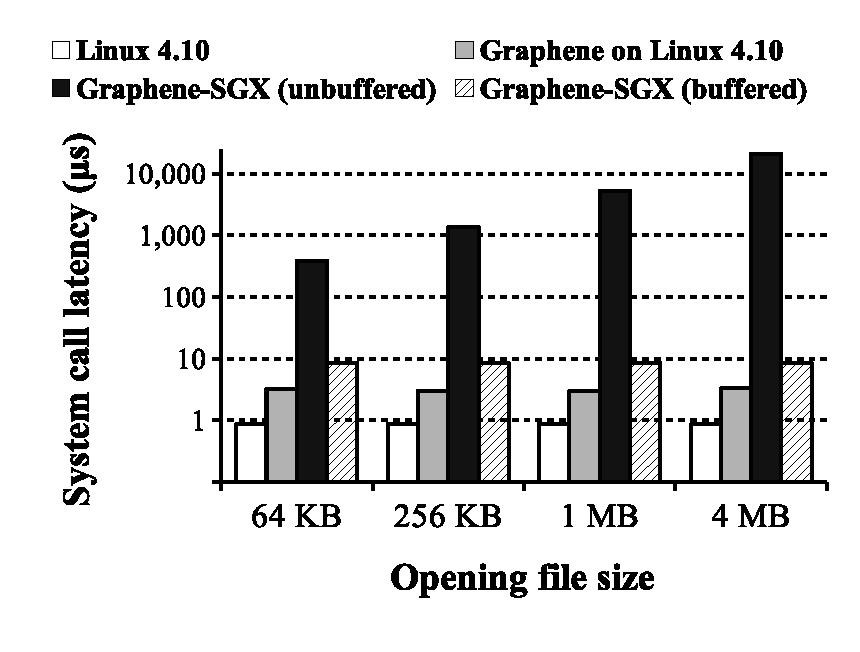
\includegraphics[height=10em]{open-latency}
\quad
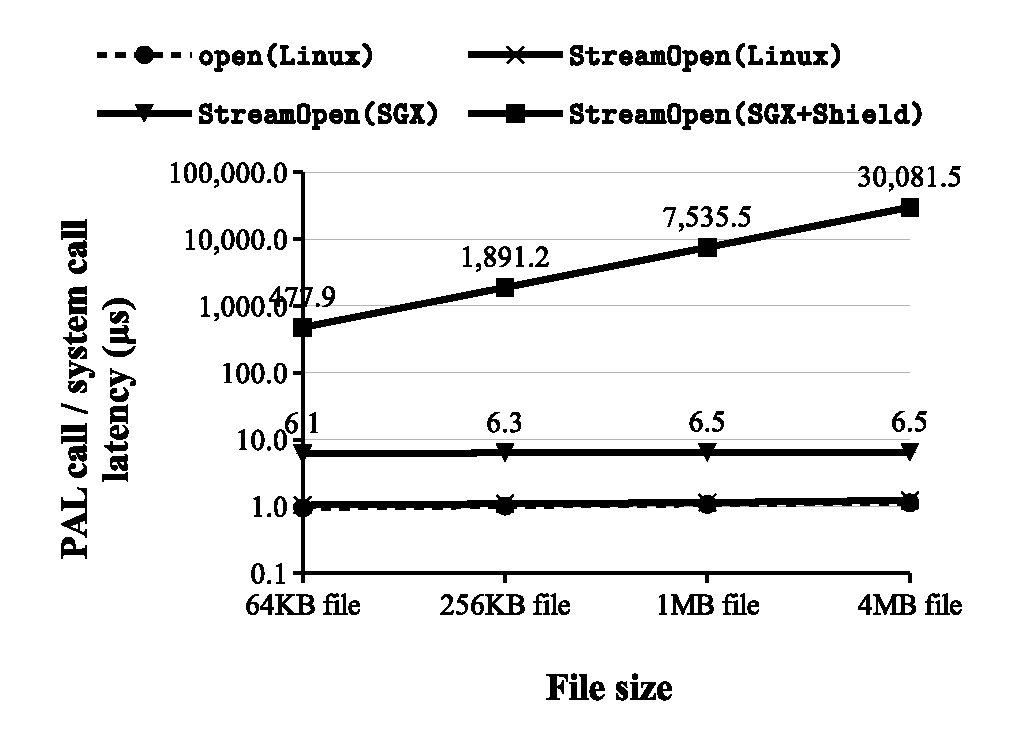
\includegraphics[height=10em]{sgx-open-latency}
}
\parbox{0.49\textwidth}{\centering\bf (a) Linux vs. Linux PAL}
\parbox{0.49\textwidth}{\centering\bf (b) Linux vs. Linux PAL vs. \sgx{} PAL}
\caption{Latency of \palcall{StreamOpen} on the Linux PAL  and \sgx{} PAL, versus \syscall{open} on Linux.
Lower is better.
Figure (a) compares \palcall{StreamOpen} on the Linux PAL,
with and without a \seccomp{} filter ({\bf +SC})
and reference monitor ({\bf +RM}), against \syscall{open} on Linux. Figure (b) compares \palcall{StreamOpen} on a \sgx{} PAL,
with and without integrity checks ({\bf +CHK}),
against the Linux PAL and \syscall{open} on Linux.}
\label{fig:eval:pal:open-latency}
\end{figure*}


Opening a file on the \sgx{} PAL
imposes significant overheads for verifying
the integrity of file contents.
Figure~\ref{fig:eval:pal:open-latency} (b) shows the latency of \palcall{StreamOpen} inside of an \sgx{} enclave, versus the latency on the Linux PAL
and in a native Linux process.
Without any security checks to shield the guest from the untrusted OS,
the latency of \palcall{StreamOpen} is dominated by the overhead of exiting the enclave and copying the argument, such as the file paths, out of the enclave.
The overheads of unshielded \palcall{StreamOpen} is 4.7--5.5$\times$, or \roughly{}5 \usec{}.
If a file is shielded with integrity protection,
\palcall{StreamOpen} will verify the checksum of the whole file against the manifest, and generate a Merkel Tree of file chunk hashes
for optimizing the latency of following \palcall{StreamRead} or \palcall{StreamMap}.
The overhead of enforcing the integrity check is correlated with the file size, and dominated by the time of
calculating a SHA256 hash of the file.
For a 4MB file, the latency of \palcall{StreamOpen} can be up to \roughly{}30 \msec{}.









\paragraph{File reads and writes.}
The latency of file reads and writes on the Linux PAL
is close to
\syscall{read} and \syscall{write}
in a Linux process.
Figure~\ref{fig:eval:pal:read-write-latency} (a) and (b) compare the latency of sequential reads and writes 
on the Linux PAL and Linux,
and show almost no overheads on the Linux PAL.
%On the Linux PAL,
%the latency of sequential reads and writes
%is correlated
%with the size of file access,
%when the size is larger than the 4KB page size.
%Besides, the latency of sequential writes is up to twice of the latency of sequential reads,
%due to the reading and writing speeds
%of the host storage.
%The latency of 
%\palcall{StreamRead} and \palcall{StreamWrite}
%on the Linux PAL
%shows a similar patterns:
%the latency is close to \syscall{read} or \syscall{write} with the size,
%with marginal overheads especially when
%the size is larger than 4KB.
The \seccomp{} filter adds a fixed overhead
around 0.06--0.09 \msec{},
which is marginal to the overall latency.
Enabling the reference monitor has nearly no overheads,
since the reference monitor only checks file paths at \palcall{StreamOpen}.
 


\begin{figure*}[t!]
\centering
\footnotesize
\resizebox{\textwidth}{!}{%
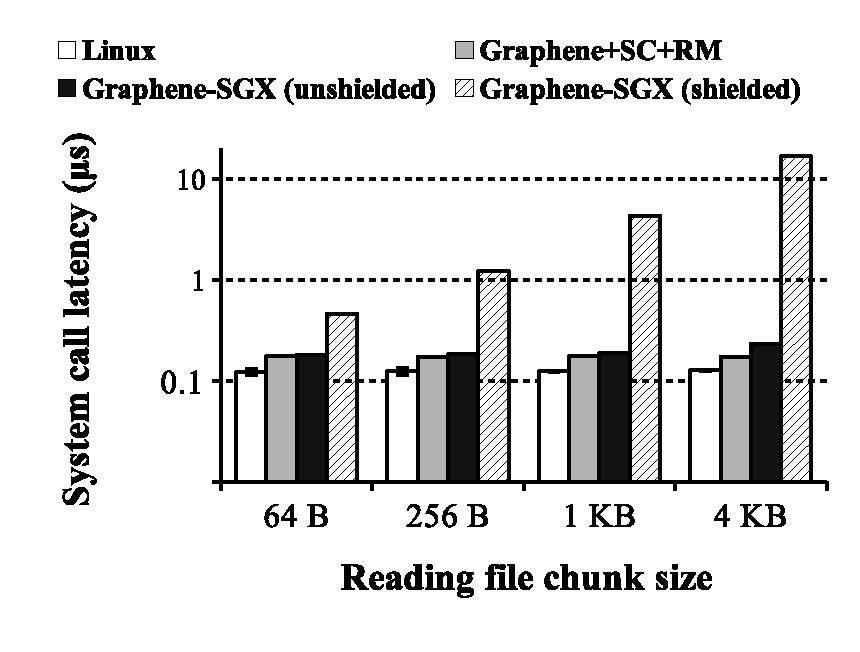
\includegraphics[height=10em]{read-latency}
\quad
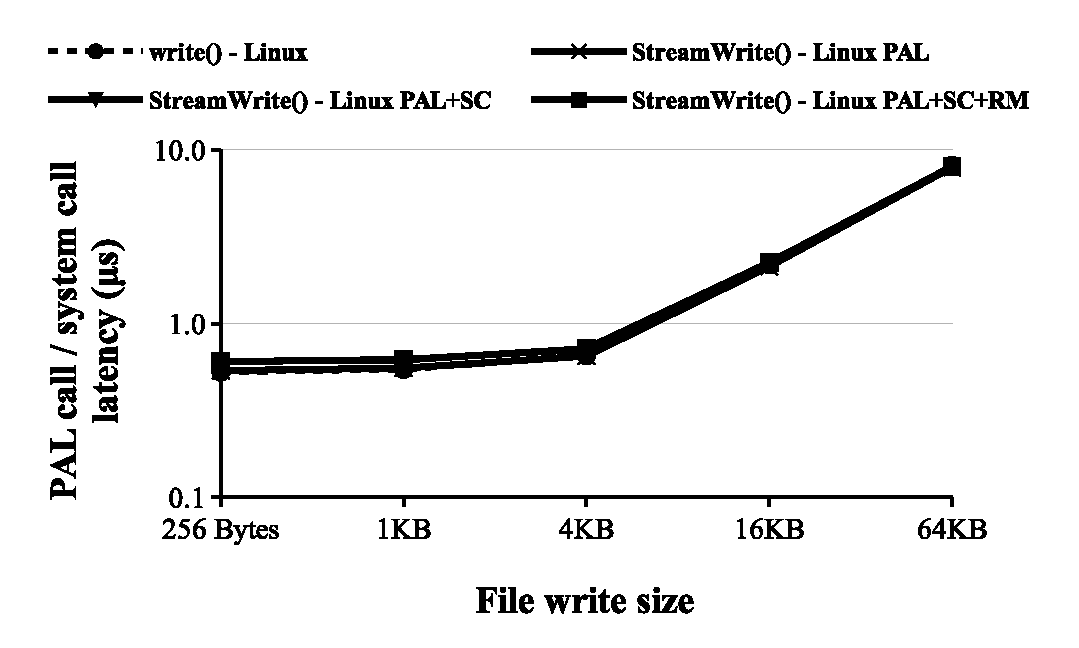
\includegraphics[height=10em]{write-latency}
}
\parbox{0.49\textwidth}{\centering\bf (a) Sequential read}
\parbox{0.49\textwidth}{\centering\bf (b) Sequential write}
\caption{Latency of sequential \palcall{StreamRead} and \palcall{StreamWrite} on the Linux PAL,
versus \syscall{read} and \syscall{write} on Linux.
Lower is better.
Figure (a) and (b) respectively compares \palcall{StreamRead} and \palcall{StreamWrite} on the Linux PAL,
with and without a \seccomp{} filter ({\bf +SC})
and reference monitor ({\bf +RM}), against \syscall{read} and \syscall{write} on Linux.}
\label{fig:eval:pal:read-write-latency}
\end{figure*}

\begin{figure*}[t!]
\centering
\footnotesize
\resizebox{\textwidth}{!}{%
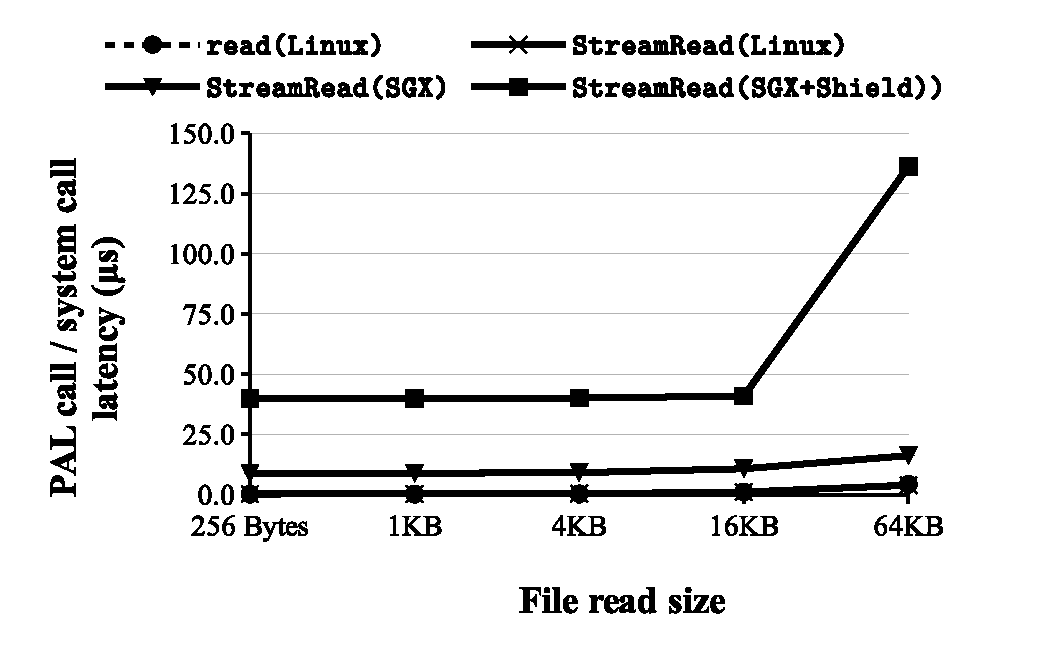
\includegraphics[height=10em]{sgx-read-latency}
\quad
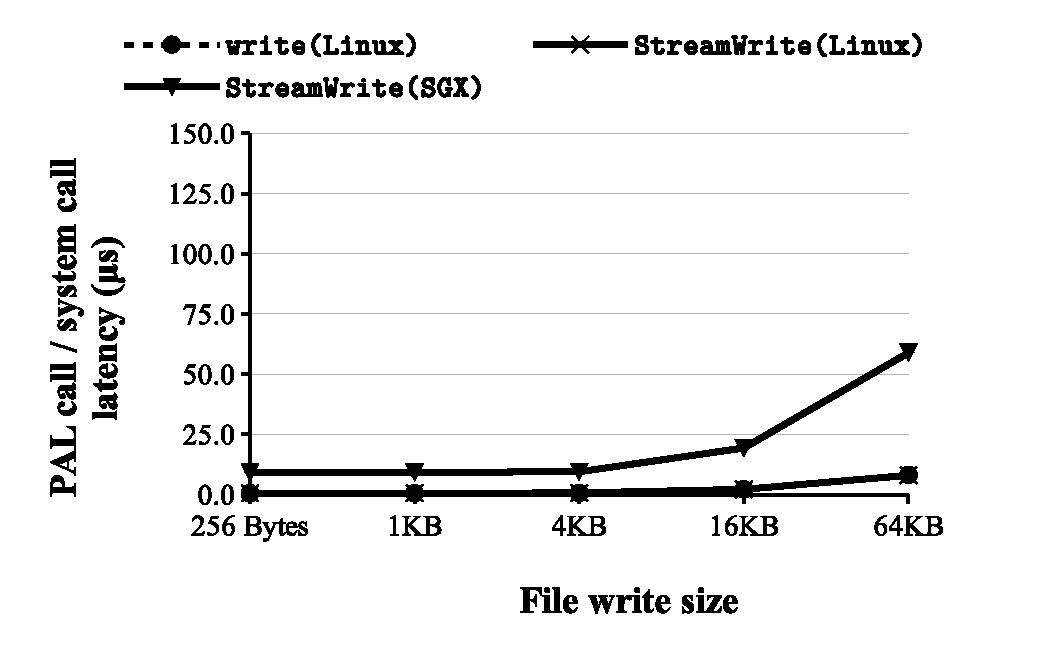
\includegraphics[height=10em]{sgx-write-latency}
}
\parbox{0.49\textwidth}{\centering\bf (a) Sequential read}
\parbox{0.49\textwidth}{\centering\bf (b) Sequential write}
\caption{Latency of sequential \palcall{StreamRead} and \palcall{StreamWrite} on the \sgx{} PAL,
versus the Linux PAL and Linux.
Lower is better.
Figure (a) and (b) respectively compares \palcall{StreamRead} and \palcall{StreamWrite} on the \sgx{} PAL,
with and without integrity checks ({\bf +CHK})
and reference monitor ({\bf +RM}), against the Linux PAL and \syscall{read} and \syscall{write} on Linux. The current design does not support integrity checks for \palcall{StreamWrite}.}
\label{fig:eval:pal:sgx-read-write-latency}
\end{figure*}


On the \sgx{} PAL,
as shown in
Figure~\ref{fig:eval:pal:sgx-read-write-latency} (a) and (b), both sequential reads and writes
have significant overheads over the latency on Linux or the Linux PAL.
The overheads contribute to:
(1) copying the contents between the enclave and the untrusted PAL; (2) cryptographic operations for 
integrity checks. Without any integrity checks,
the cost of exiting the enclave
and copying the contents across the enclave boundary is
8--12 \usec{} for reads and 8--50 \usec{} for writes.
If the \sgx{} PAL checks the integrity of file contents
at file reads,
the latency is bounded by
the cost of copying 16KB blocks into the enclave
and calculating the secure hashes to compare with the Merkle tree.
Reducing the hashing size from 16KB to even smaller block
will improve
the latency of small reads,
but also will increase the size of Merkle tree.
The experiment does not measure the overhead of integrity protection on file writes
because the feature is not yet implemented
in the \sgx{} PAL.








%\paragraph{Network connections.}



\begin{figure*}[t!]
\centering
\footnotesize
\resizebox{\textwidth}{!}{%
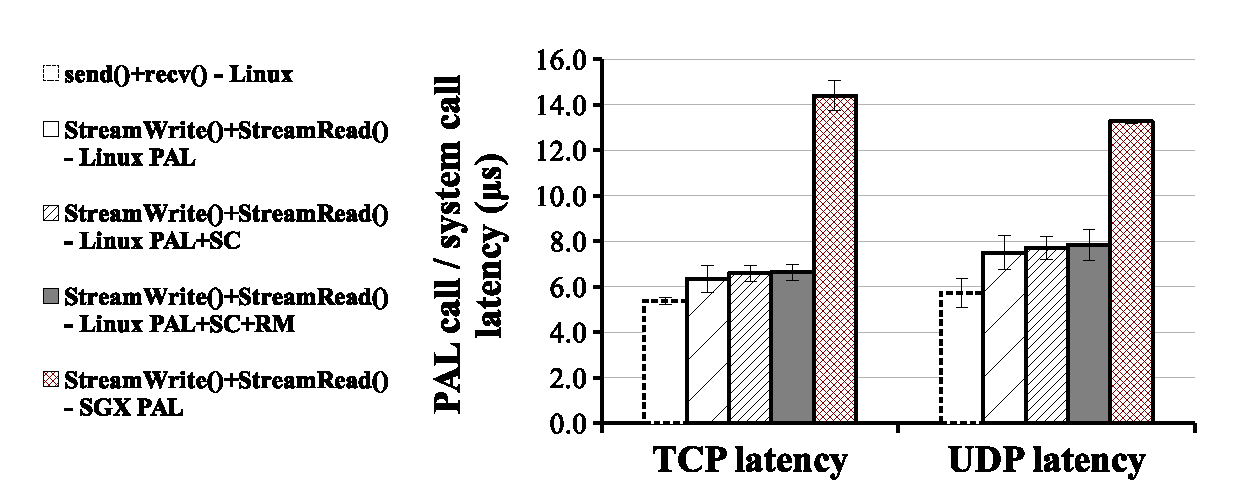
\includegraphics[height=10em]{tcp-udp-latency}
\quad
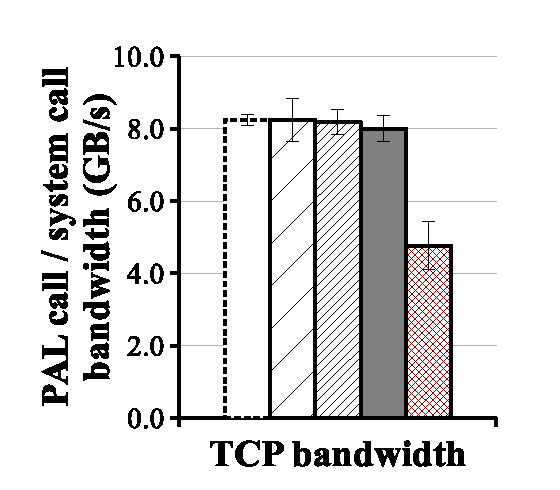
\includegraphics[height=10em]{tcp-bandwidth}
}
\parbox{0.24\textwidth}{\quad}
\parbox{0.49\textwidth}{\centering\bf (a) Latency ({\usec})}
\parbox{0.24\textwidth}{\centering\bf (b) Bandwidth (MB/\asec{})}
\caption{(a) Latency of sending a short message over TCP and UDP sockets (lower is better), and (b) bandwidth of sending large data over TCP (higher is better).
The comparison is between (1) \syscall{recv} and \syscall{send} on Linux; (2) \palcall{StreamRead} and \palcall{StreamWrite} on a Linux PAL, with and without a \seccomp{} filter ({\bf +SC}) and reference monitor ({\bf +RM}); (3) the same \hostapis{} on the \sgx{} PAL, without data protection.}
\label{fig:eval:pal:network-latency-bandwidth}
\end{figure*}



\paragraph{TCP and UDP sockets.}
%The evaluation shows both the latency and bandwidth of sending and receiving messages over a TCP or UDP sockets.
The Linux PAL imposes \roughly{}18\% and \roughly{}30\% overheads
on the latency of TCP and UDP sockets (bound on localhost),
respectively,
as shown in
Figure~\ref{fig:eval:pal:network-latency-bandwidth} (a).
The overheads specifically contribute
to cost of translating to \syscall{sendmsg} and \syscall{recvmsg}
in the Linux host,
which requires passing a data structure
containing buffer pointer, size, and a socket address
for UDP messaging. 
The UDP socket address is also checked by the reference monitor if enabled, adding extra overheads to the \hostapis{}.
Figure~\ref{fig:eval:pal:network-latency-bandwidth} (b)
also shows the bandwidth of TCP sockets
for sending 64KB messages locally,
which has only 4\% overheads on the Linux PAL.
In addition, both the \seccomp{} filter and reference monitor
cause less than 1\% overheads
on TCP bandwidth.



% shows the turnaround time of sending single-byte messages back and forth over a TCP or UDP stream (connected through the local loopback device), and
%Figure~\ref{fig:eval:pal:network-latency-bandwidth} (b)
%shows the bandwidth of a TCP or UDP stream
%to transfer
%64KB messages between \picoprocs{}.
%On the Linux PAL,
%the overheads of ping-ponging over TCP or UDP primarily contribute to the translation cost between
%the \hostapis{} to Linux system calls (specifically, \syscall{sendmsg} and \syscall{recvmsg}),
%since the the \hostapis{} use strings as the network URIs and the Linux system calls take a network address structure (\code{struct sockaddr}) that contains numeric representations in integers.
%The translation costs for a TCP stream and a UDP stream are \roughly{}18\% and \roughly{}30\%, respectively.
%The overhead is relatively marginal in the TCP bandwidth test,
%at \roughly{}4\%.
%Both the \seccomp{} filter and reference monitor adds
%a marginal, less than 1\% overhead
%to either the latency or bandwidth of TCP or UDP sockets.


TCP and UDP sockets on the \sgx{} PAL
also have significant overheads compared to the Linux PAL,
due to the cost of enclave interface.
As shown in
both Figure~\ref{fig:eval:pal:network-latency-bandwidth}
(a) and (b),
the overheads of the \sgx{} PAL on TCP and UDP latency
are \roughly{}167\% and \roughly{}131\%,
respectively; the overhead on TCP bandwidth also reaches \roughly{}79\%. 
Note that the current design
of the \sgx{} PAL does not protect the messages sent or received
over a TCP or UDP socket.
The decision is based on previous work~\cite{osdi16scone},
which concludes that
inline encryption and authentication inside applications
is more efficient
than shielding at the enclave interface
or the system interface.
\graphenesgx{} makes the assumption
that most networked applications have adopted SSL/TLS
to protect the confidentiality and integrity of network payloads.



\begin{figure*}[t!]
\centering
\footnotesize
\resizebox{\textwidth}{!}{%
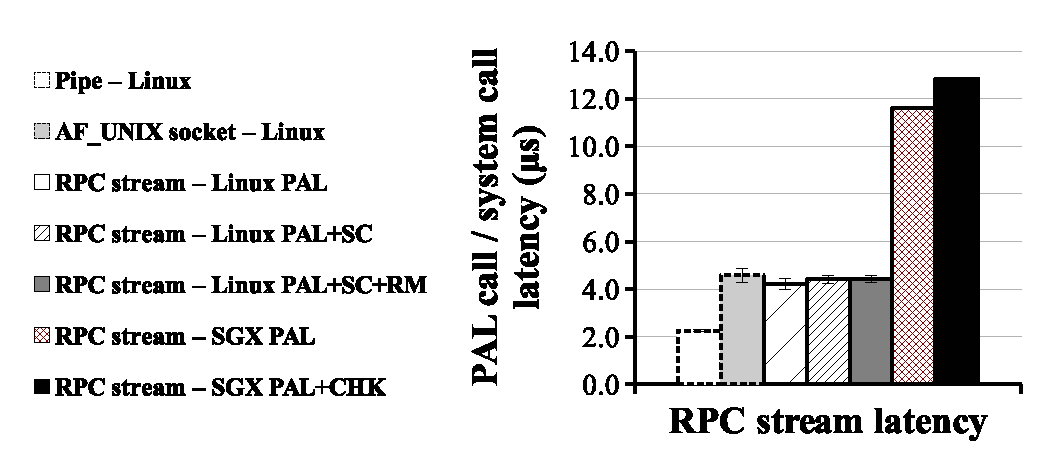
\includegraphics[height=10em]{pipe-latency}
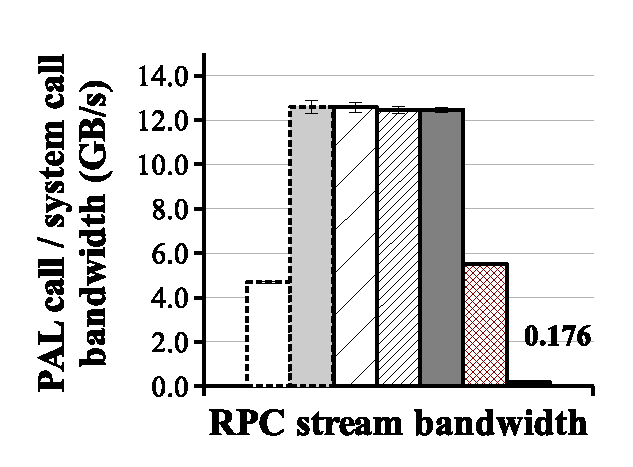
\includegraphics[height=10em]{pipe-bandwidth}
}
\parbox{0.30\textwidth}{\quad}
\parbox{0.34\textwidth}{\centering\bf (a) Latency ({\usec})}
\parbox{0.34\textwidth}{\centering\bf (b) Bandwidth (MB/\asec{})}
\caption{(a) Latency of sending a short message over RPC (lower is better), and (b) bandwidth of sending large data (higher is better).
The comparison is between (1) \syscall{read} and \syscall{write} over a pipe or an AF\_UNIX socket on Linux; (2) \palcall{StreamRead} and \palcall{StreamWrite} on the Linux PAL, with and without a \seccomp{} filter ({\bf +SC}) and reference monitor ({\bf +RM}); (3) the same \hostapis{} on the \sgx{} PAL, with and without data protection ({\bf +CHK}).}
\label{fig:eval:pal:pipe-latency-bandwidth}
\end{figure*}



\paragraph{RPC latency and bandwidth.}
%The evaluation shows the latency and bandwidth of using a RPC stream to send messages across \picoprocs{}.
Due to the choice of underlying abstraction,
both the latency and bandwidth
of a RPC stream on the Linux PAL is close to a UNIX domain socket
on native Linux kernel.
Figure~\ref{fig:eval:pal:pipe-latency-bandwidth} (a)
compares
the latency of sending one-byte messages
over a local RPC stream,
a pipe, and a UNIX domain socket (the last two are both in a native Linux process).
The results
show that the latency of a UNIX domain socket
is about twice as slow as a pipe,
and close to the latency of a RPC stream
on the Linux PAL,
with or without the \seccomp{} filter and reference monitor.
Figure~\ref{fig:eval:pal:pipe-latency-bandwidth} (b)
also shows the bandwidth
of messaging over a RPC stream, a UNIX domain socket,
and a pipe,
and first two reach bandwidth
more than double of the pipe bandwidth.
Both the \seccomp{} filter and reference monitor introduce marginal overheads (less than 5\%) to RPC latency and bandwidth.
Note that this performance pattern is specific
to kernels after 4.2; a zero-copy design for UNIX domain socket
is adopted in Linux 4.2,
and makes a UNIX domain socket
almost equally fast as the bulk IPC abstraction
in the Linux PAL
(see Section~\ref{sec:eval:pal:multi-proc}). 



For the \sgx{} PAL,
the fundamental cost of enclave exits and copying message contents,
without protecting the message contents,
is \roughly{}154\% to the latency,
or \roughly{}127\% to the bandwidth.
Unlike network sockets, 
applications generally assume transferring data over a local pipe or FIFO to be secure on a trusted host, and do not enforce protection like SSL/TLS.
%\graphenesgx{} cannot assume RPC streams to be protected by SSL/TLS in applications.
%Since it is likely that an application may send sensitive information
%over a pipe or a UNIX socket,
%the underlying RPC streams must always be protected by the \sgx{} PAL.
For each RPC stream, the \sgx{} PAL establishes a TLS connection using a 256-bits AES-GCM algorithm, which both authenticates and encrypts the message contents.
The AES-GCM algorithm is accelerated by the Intel AES-NI instructions, which exist on all \sgx{}-enabled CPUs.
With the hardware acceleration,
when sending one-byte messages,
the overhead on RPC latency is \roughly{}10\% compared to the UNIX domain socket;
furthermore, RPC bandwidth of sending large messages
is reduced by \roughly{}31$\times$, at \roughly{}0.176 GB/s.
Switching to a more efficient cryptographic algorithm or library may improve the efficiency of RPC streams,
and such experiments are left for future work.






\paragraph{Summary.}
According to the evaluation, the overheads on accessing a file or an I/O stream
with one of the PAL design
contribute to translation cost of \thehostabi{} semantics
and the reference monitor.
Because a file or an I/O stream
is shareable among \picoprocs{}, the reference monitor
must check the access, at least
at opening the file or the I/O stream.

%due to the nature of these abstractions to be sharable
%among applications.
%Each of these \hostapis{} externalizes certain guest OS states
%%such as buffered file contents or network payloads,
%to the host OS,
%using the existing host system interfaces.
%Most of the experiment results
%show that the translation cost between the \hostapis{} and the host system interfaces can be reduced
%by mitigating the needs of reconstructing the \hostapi{} arguments
%and copying stream buffers.
%Only a few exceptions, such as the translation of URIs to network addresses,
%or copying the arguments or buffers in or out of an enclave,
%cause more significant overheads to the overhead of these system calls.




Security checks, either in the host kernel or inside an enclave,
often contribute to
non-trivial overheads on the \hostapis{} for accessing I/O streams.
The cost of security checks
varies between different threat models.
For the Linux PAL, the cost includes the overhead of enabling a \seccomp{} filter, and the cost of checking file paths and network addresses
inside of an reference monitor.
With the JIT (Just-in-time) optimization,
the overheads of \seccomp{} filter is generally less than 10\%.
The overheads of security monitors can range from 0--21\%, but only impact \hostapis{} which accept an URI as argument (e.g., \palcall{StreamOpen} and \palcall{StreamAttrQuery}).

 
The \sgx{} PAL further adopts several cryptographic techniques
for protecting the confidentiality and integrity of I/O streams, and cryptographic operations tend to cause significant overheads.
Verifying the file contents, either at first open of the file or consequential file reads,
causes 500--24,000$\times$ overheads on \palcall{StreamOpen}
or 25--150$\times$ overheads on \palcall{StreamRead}.
Authenticating and encrypting a RPC stream with a hardware-accelerated AES-GCM algorithm
causes up to 335\% overheads on latency in comparison with
the underlying UNIX domain sockets,
or up uo \roughly{}20 $\times$ overhead on bandwidth.


